\titleformat{\chapter}[display]
{\normalfont\huge\bfseries}{Capítulo \thechapter}{0.5em}{\huge}
\titlespacing*{\chapter}{0pt}{-1.25cm}{25pt}
\chapter{Contexto del problema y estado del arte}

\section{Contexto del problema}

El \textit{Automatic Packet Reporting System} (APRS) como sistema de comunicación digital se basa en la gran comunidad de radioaficionados e incluso tiene aplicaciones industriales como la transmisión de información en tiempo real de vehículos logísticos o estaciones de meteorología. A pesar de su versatilidad y flexibilidad, el APRS presenta algunas barreras de entrada para usuarios que no pertenecen a la comunidad radioaficionada o tienen sólidos conocimientos de este ámbito. En este capítulo, se analizarán estas barreras y se discutirán los requisitos necesarios.

\subsection{Barreras de entrada}

El APRS requiere conocimientos básicos sobre radiocomunicación y la obtención de una licencia de radioaficionado en caso de querer emitir. La obtención de la licencia a pesar de no implicar un desembolso económico importante, si que requiere un estudio y comprensión de los sistemas y legislación pertinente.

Adicionalmente, el APRS utiliza una estructura de mensaje específico y un conjunto de protocolos que pueden ser difíciles de entender para usuarios no familiarizados con este tipo de tecnología. La falta de documentación y antigüedad de esta hacen que desarrollar soluciones para este sistema sea complicado.

\subsection{Hardware}

Para utilizar APRS, se necesita hardware especializado que incluya un transceptor de radio, un \textit{Terminal Node Controller} (TNC) y un dispositivo GPS (opcionalmente), existen otras opciones más baratas como los dispositivos \textit{software defined radio} o RTL-SDR \Cref{fig:rtl-sdr} que se conectan directamente a un ordenador. Los TNC son dispositivos que convierten las señales digitales emitidas por un ordenador en señales de radio y viceversa. El dispositivo GPS proporciona información de ubicación que se puede transmitir junto con otros datos en el cuerpo del mensaje.

El precio del hardware APRS puede variar dependiendo de la calidad y las características del equipo. Sin embargo, a pesar de no contar con precios prohibitibamente altos, la inversión que supone conlleva el hecho de que solamente los usuarios con un interés previo en la radioafición o la tecnología en general estén dispuestos a adquirirlo.

\begin{figure}
    \centering
    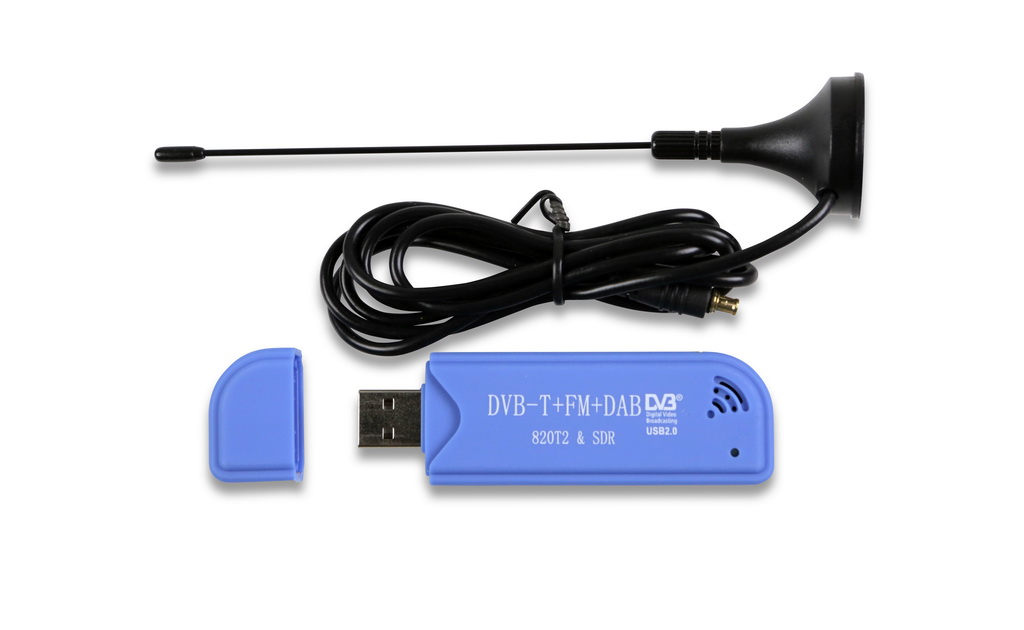
\includegraphics[width=0.5\textwidth]{Imagenes/Chapter_2/rtl_sdr.jpg}
    \caption{Ejemplo de un RTL-SDR de tipo usb.}
    \label{fig:rtl-sdr}
\end{figure}


\subsection{OSINT y APRS}

El APRS sirve como una herramienta de comunicación para los radioaficionados y de reporte de telemetría para las industrias. Pero se puede convertir en una valiosa fuente de información para la obtención de inteligencia (OSINT). Esto se debe a su capacidad para proporcionar una gran cantidad de datos en tiempo real sobre ubicación y estado de los activos así como una amplia gama de información adicional.

En el ámbito del OSINT, el APRS ofrece una serie de aplicaciones prácticas. Por ejemplo, los datos APRS son actualmente utilizados para el rastreo de vehículos en tiempo real, lo que resulta muy útil para empresas de logística y transporte. Además, la red APRS se utiliza para monitorear la actividad de estaciones meteorológicas, proporcionando datos en tiempo real sobre condiciones climáticas locales. También se utiliza en situaciones de emergencia, como pueden ser desastres naturales o incidentes críticos, el APRS desempeña un papel crucial al permitir la transmisión rápida de información sobre ubicaciones de refugios, recursos disponibles y necesidades de ayuda, ya que no depende necesariamente de infraestructura de una entidad como si lo hace la red telefónica.

Aunque el APRS tiene un gran potencial para aplicaciones en el ámbito del OSINT, su uso en esta área es prácticamente inexistente. Este hecho puede explicarse en parte por las barreras de entrada mencionadas anteriormente, que incluyen la necesidad de poseer conocimientos especializados en radiocomunicación, obtener licencias de radioaficionado y adquirir hardware especializado.

\section{Estado del Arte}

Existen varios sitios web que ofrecen servicios relacionados con APRS, entre los cuales destacan \textbf{aprs.fi} y \textbf{aprs.to} probablemente las dos webs más grandes.

\subsection{aprs.fi}

aprs.fi es una de las webs más utilizadas para visualizar datos APRS en tiempo real y acceder a un histórico extenso de información. Sin embargo, su interfaz puede considerarse un tanto desactualizada (ver \Cref{fig:aprs-fi}), lo que puede dificultar la navegación y la búsqueda de información específica. Aunque ofrece una gran cantidad de datos y un histórico significativo, la plataforma carece de capacidades avanzadas de filtrado de estaciones y mensajes. Además, para acceder a funciones más complejas y realizar extracciones de datos, es necesario crear una cuenta.

\begin{figure}[h]
    \centering
    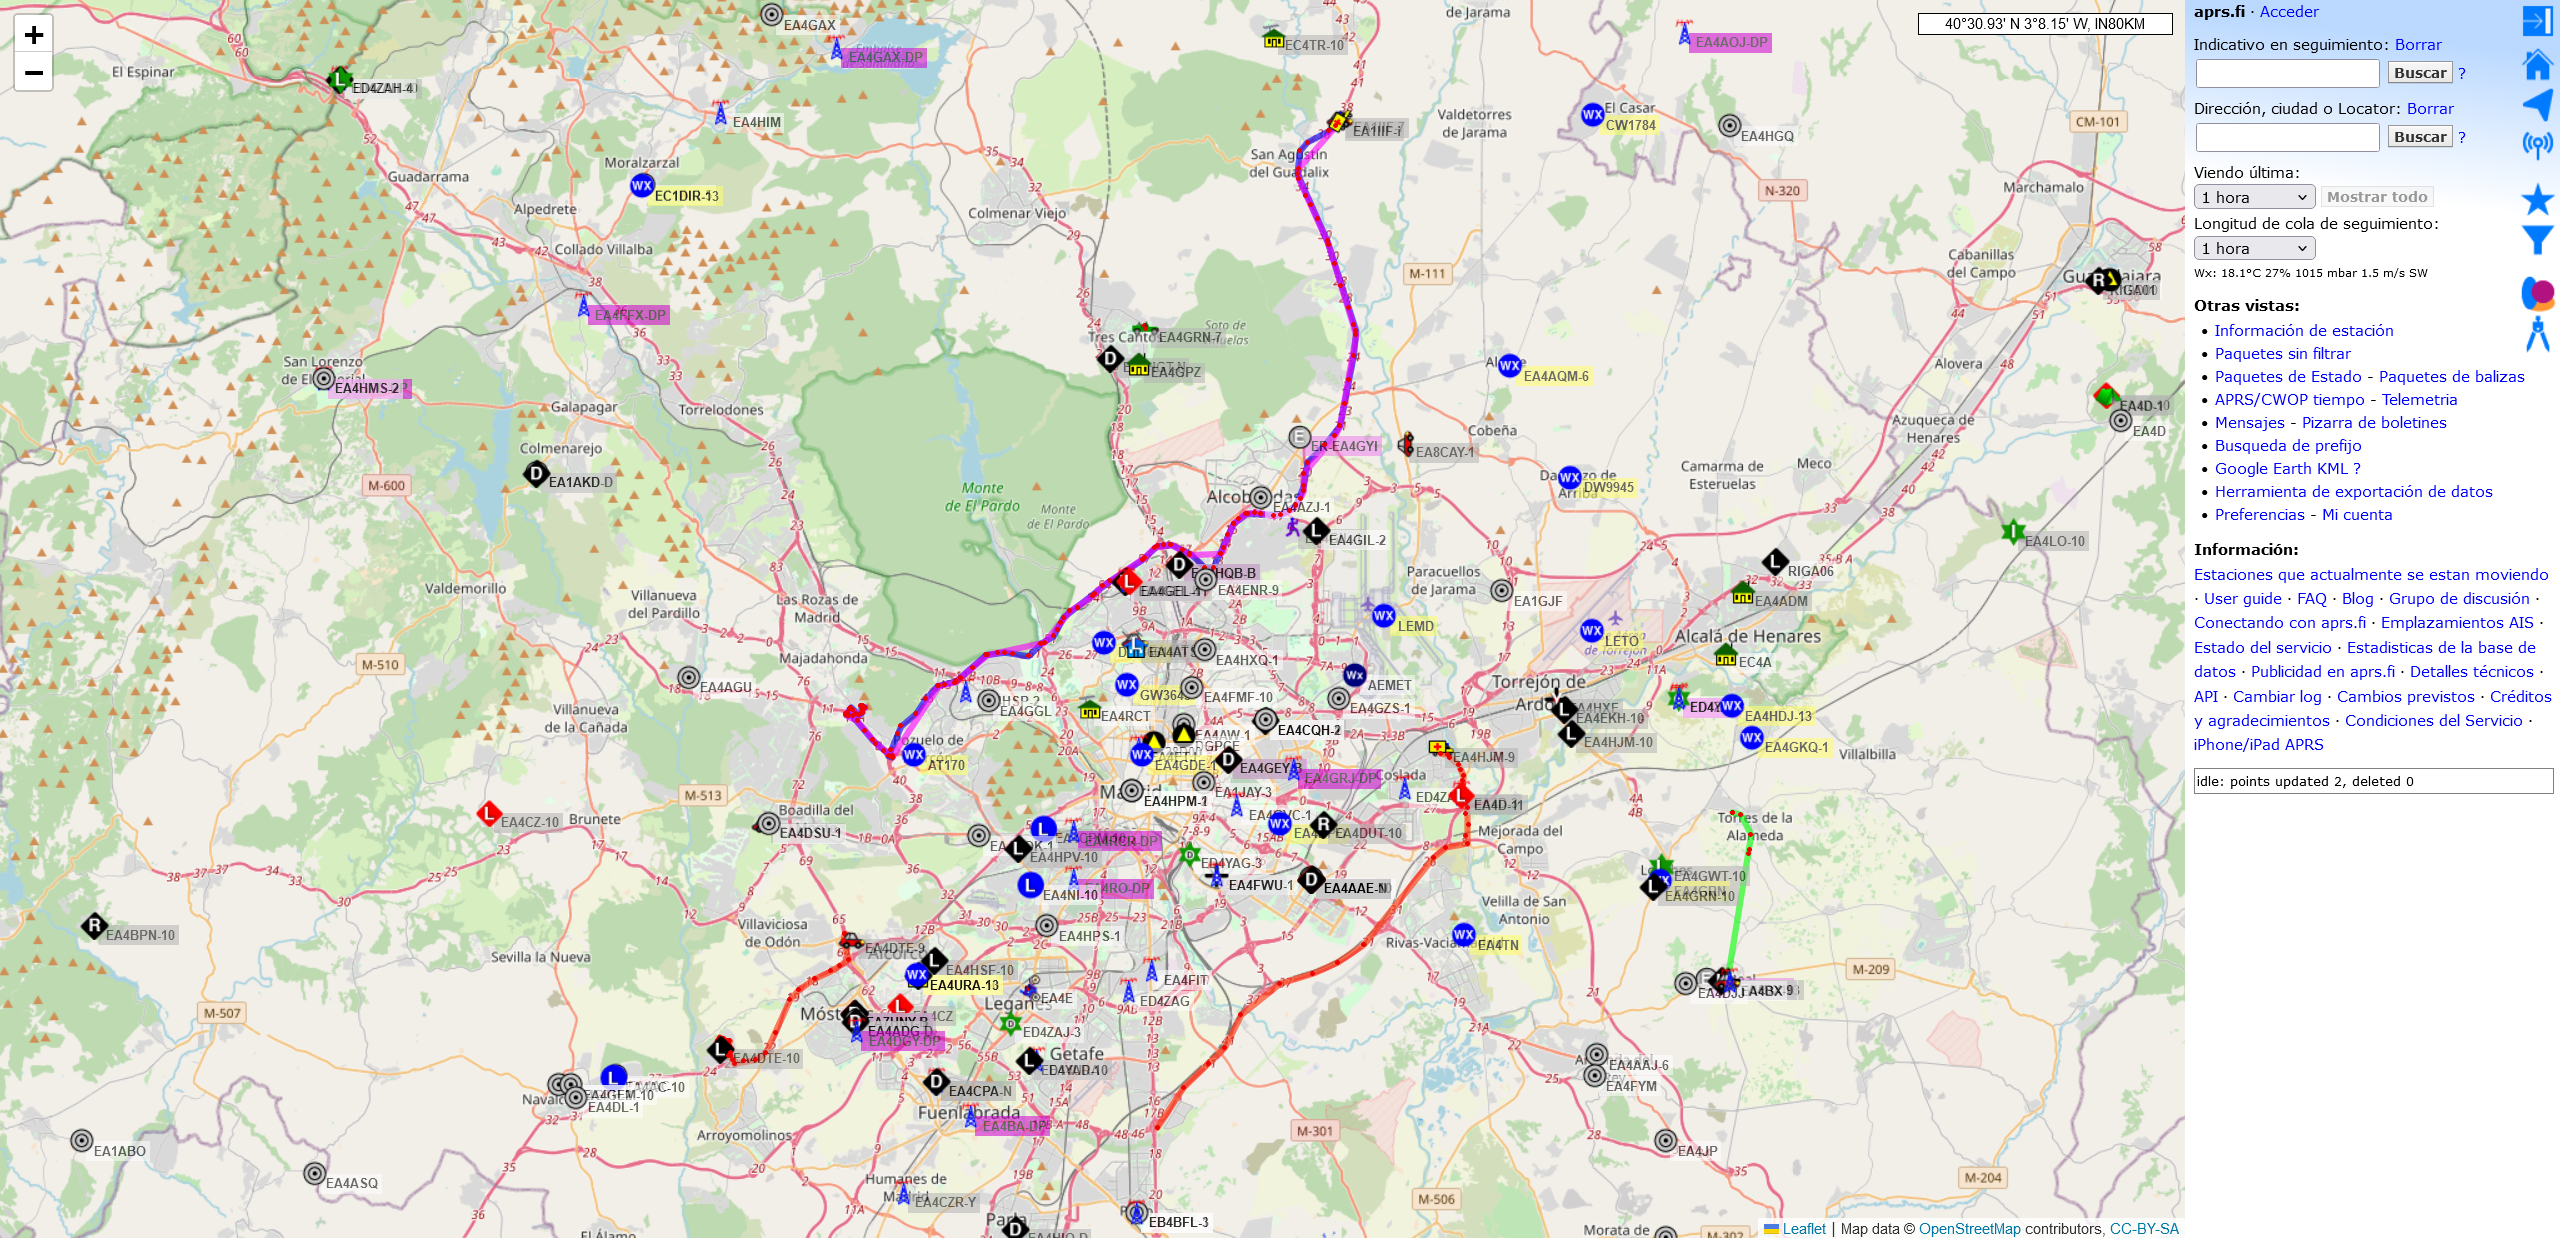
\includegraphics[width=0.7\textwidth]{Imagenes/Chapter_2/aprs-fi.png}
    \caption{Interfaz de aprs.fi}
    \label{fig:aprs-fi}
\end{figure}

\subsection{aprs.to}

Por otro lado, aprs.to ofrece una interfaz más moderna y cuidada (ver \Cref{fig:aprs-to}), lo que facilita la navegación y la búsqueda de información. Además, permite realizar búsquedas básicas y aplicar filtros para refinar los resultados. Sin embargo, al igual que aprs.fi, también requiere que los usuarios se creen una cuenta para acceder a ciertas funcionalidades avanzadas.

\begin{figure}[h]
    \centering
    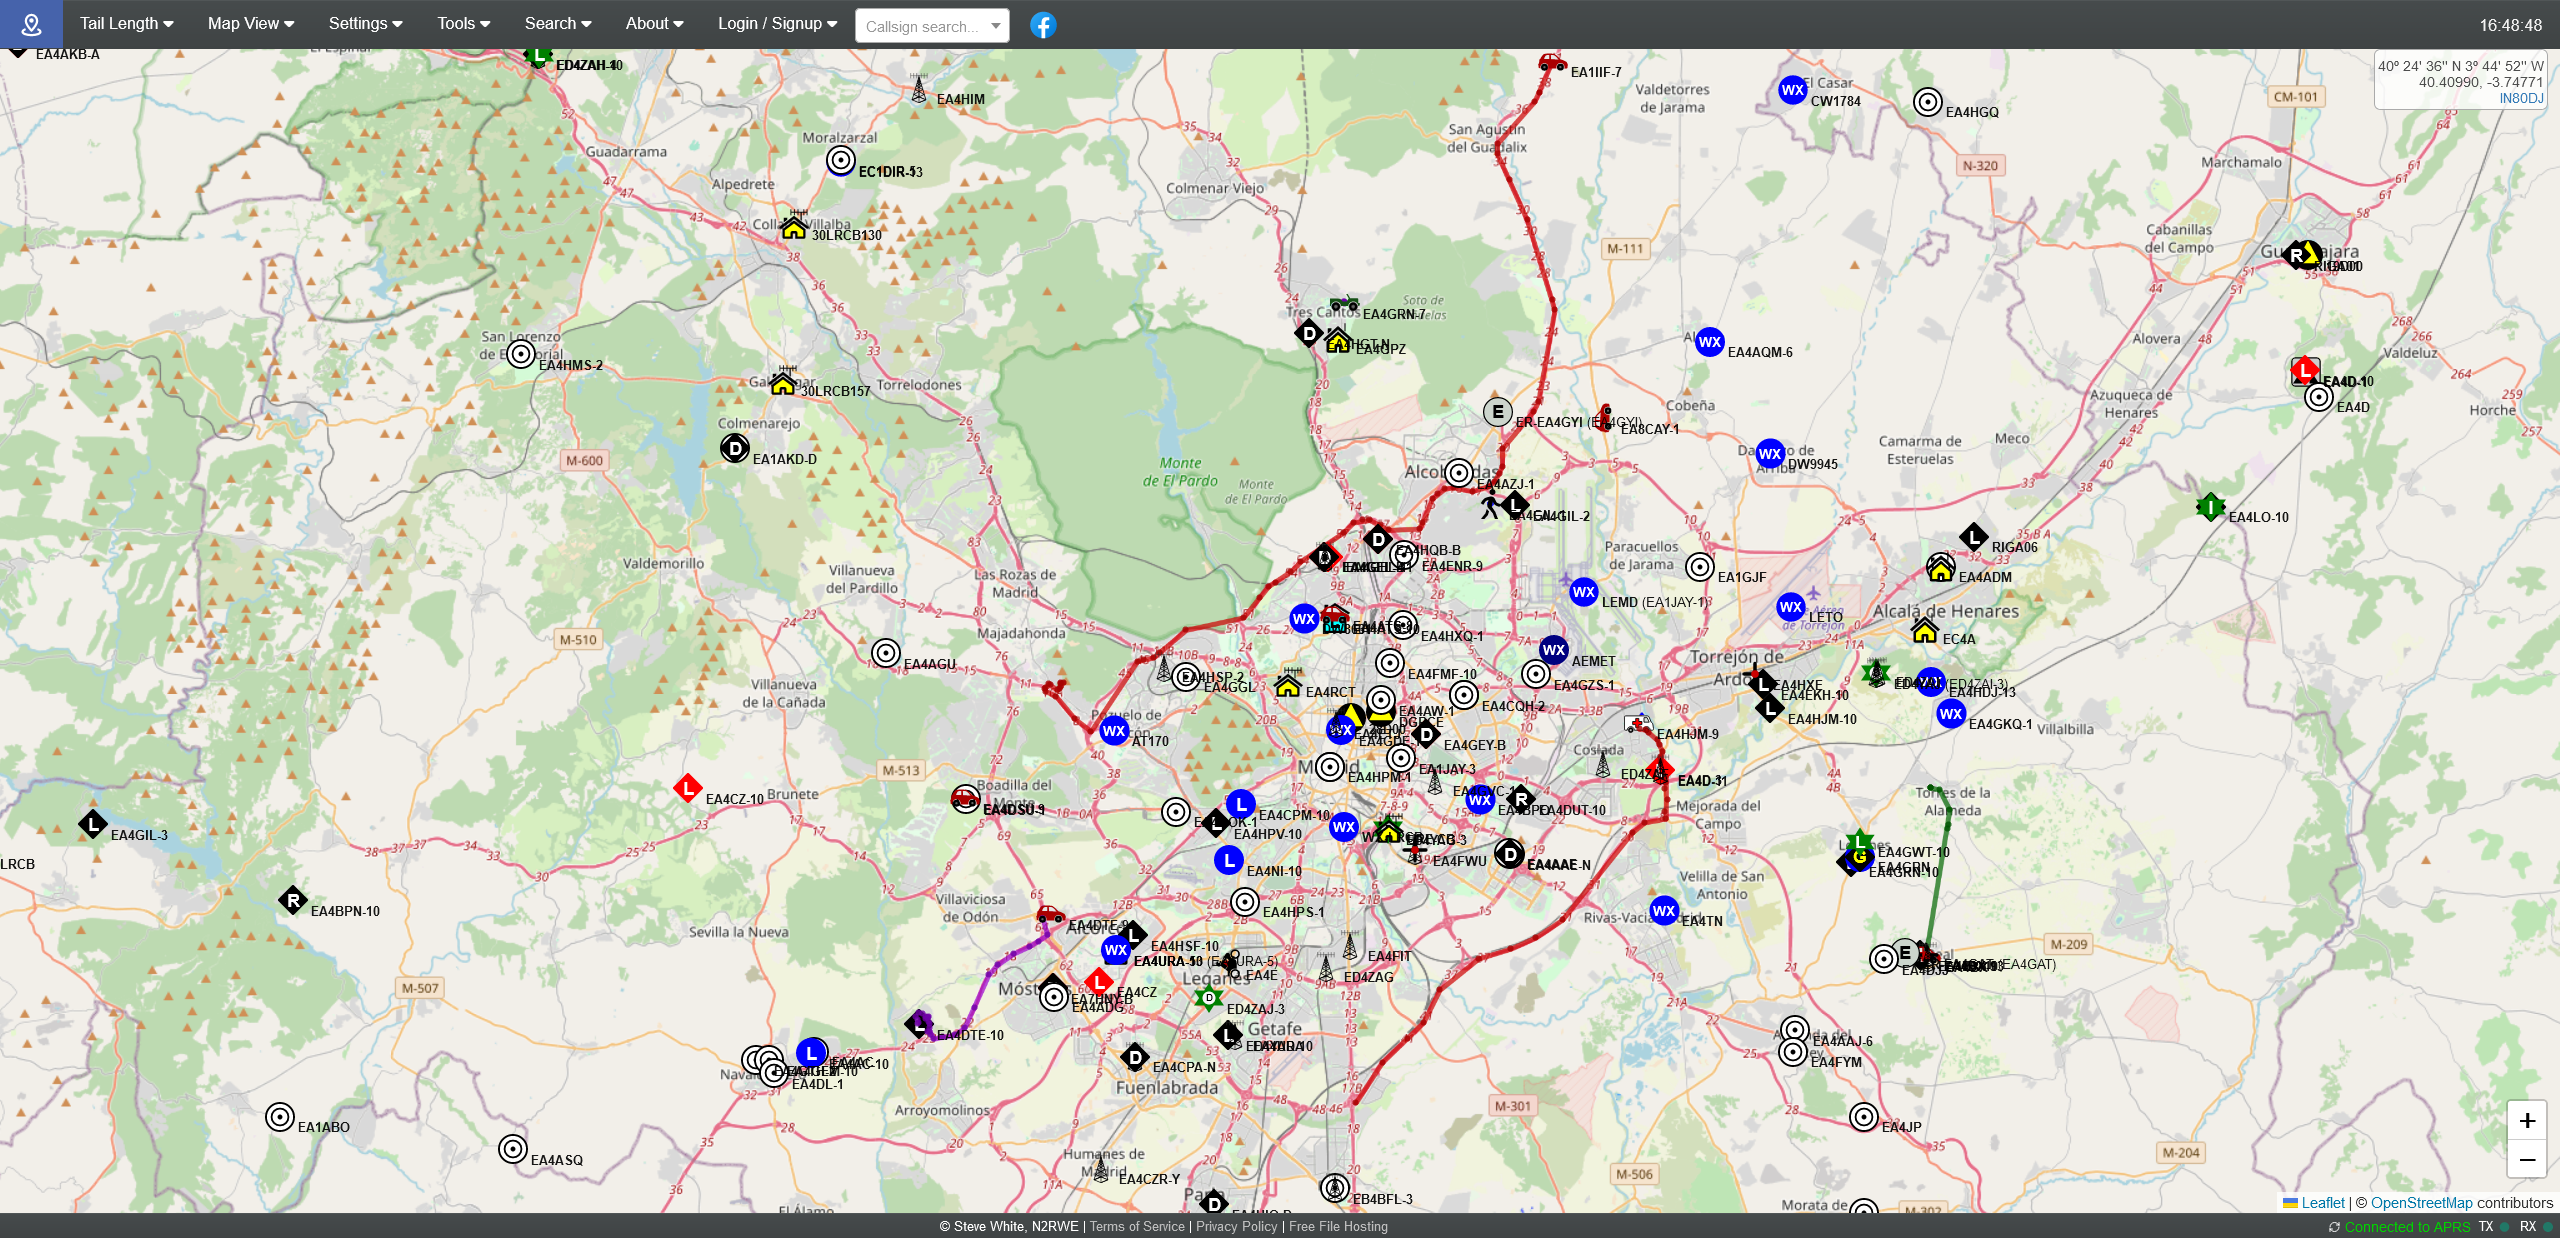
\includegraphics[width=0.7\textwidth]{Imagenes/Chapter_2/aprs-to.png}
    \caption{Interfaz de aprs.to}
    \label{fig:aprs-to}
\end{figure}

\subsection{Comparación}

En resumen, aprs.fi, la web de visualización de APRS por excelencia, ofrece una gran base de datos y una gran cantidad de información histórica de datos APRS, pero su interfaz puede resultar algo desactualizada y carece de capacidades avanzadas de filtrado. Por otro lado, aprs.to presenta una interfaz más moderna y permite realizar búsquedas básicas y aplicar filtros, aunque también requiere crear una cuenta para acceder a ciertas funciones. Ambas plataformas tienen puntos fuertes y débiles y por esa razón lo mejor es usarlas en conjunto.


\section{APRSINT}
La solución propuesta se ha llamado \textbf{APRSINT}, que es una combinación de APRS y OSINT. APRSINT está dividida en tres módulos principales:
\begin{itemize}
	\item \textbf{Adquisición de Datos:} Este módulo se encargará de recopilar y almacenar los mensajes APRS de diversas fuentes, así como de integrar datos de otras fuentes abiertas y disponibles.
	\item \textbf{Procesamiento y Análisis:} Este módulo se encargará de procesar y analizar los datos recopilados, ofreciendo herramientas avanzadas de visualización, filtrado y análisis de datos.
	\item \textbf{Visualización y Presentación:} Este módulo se encargará de presentar los datos procesados y analizados de forma clara y comprensible, facilitando la interpretación y la toma de decisiones.
\end{itemize}

\begin{figure}[h]
    \centering
    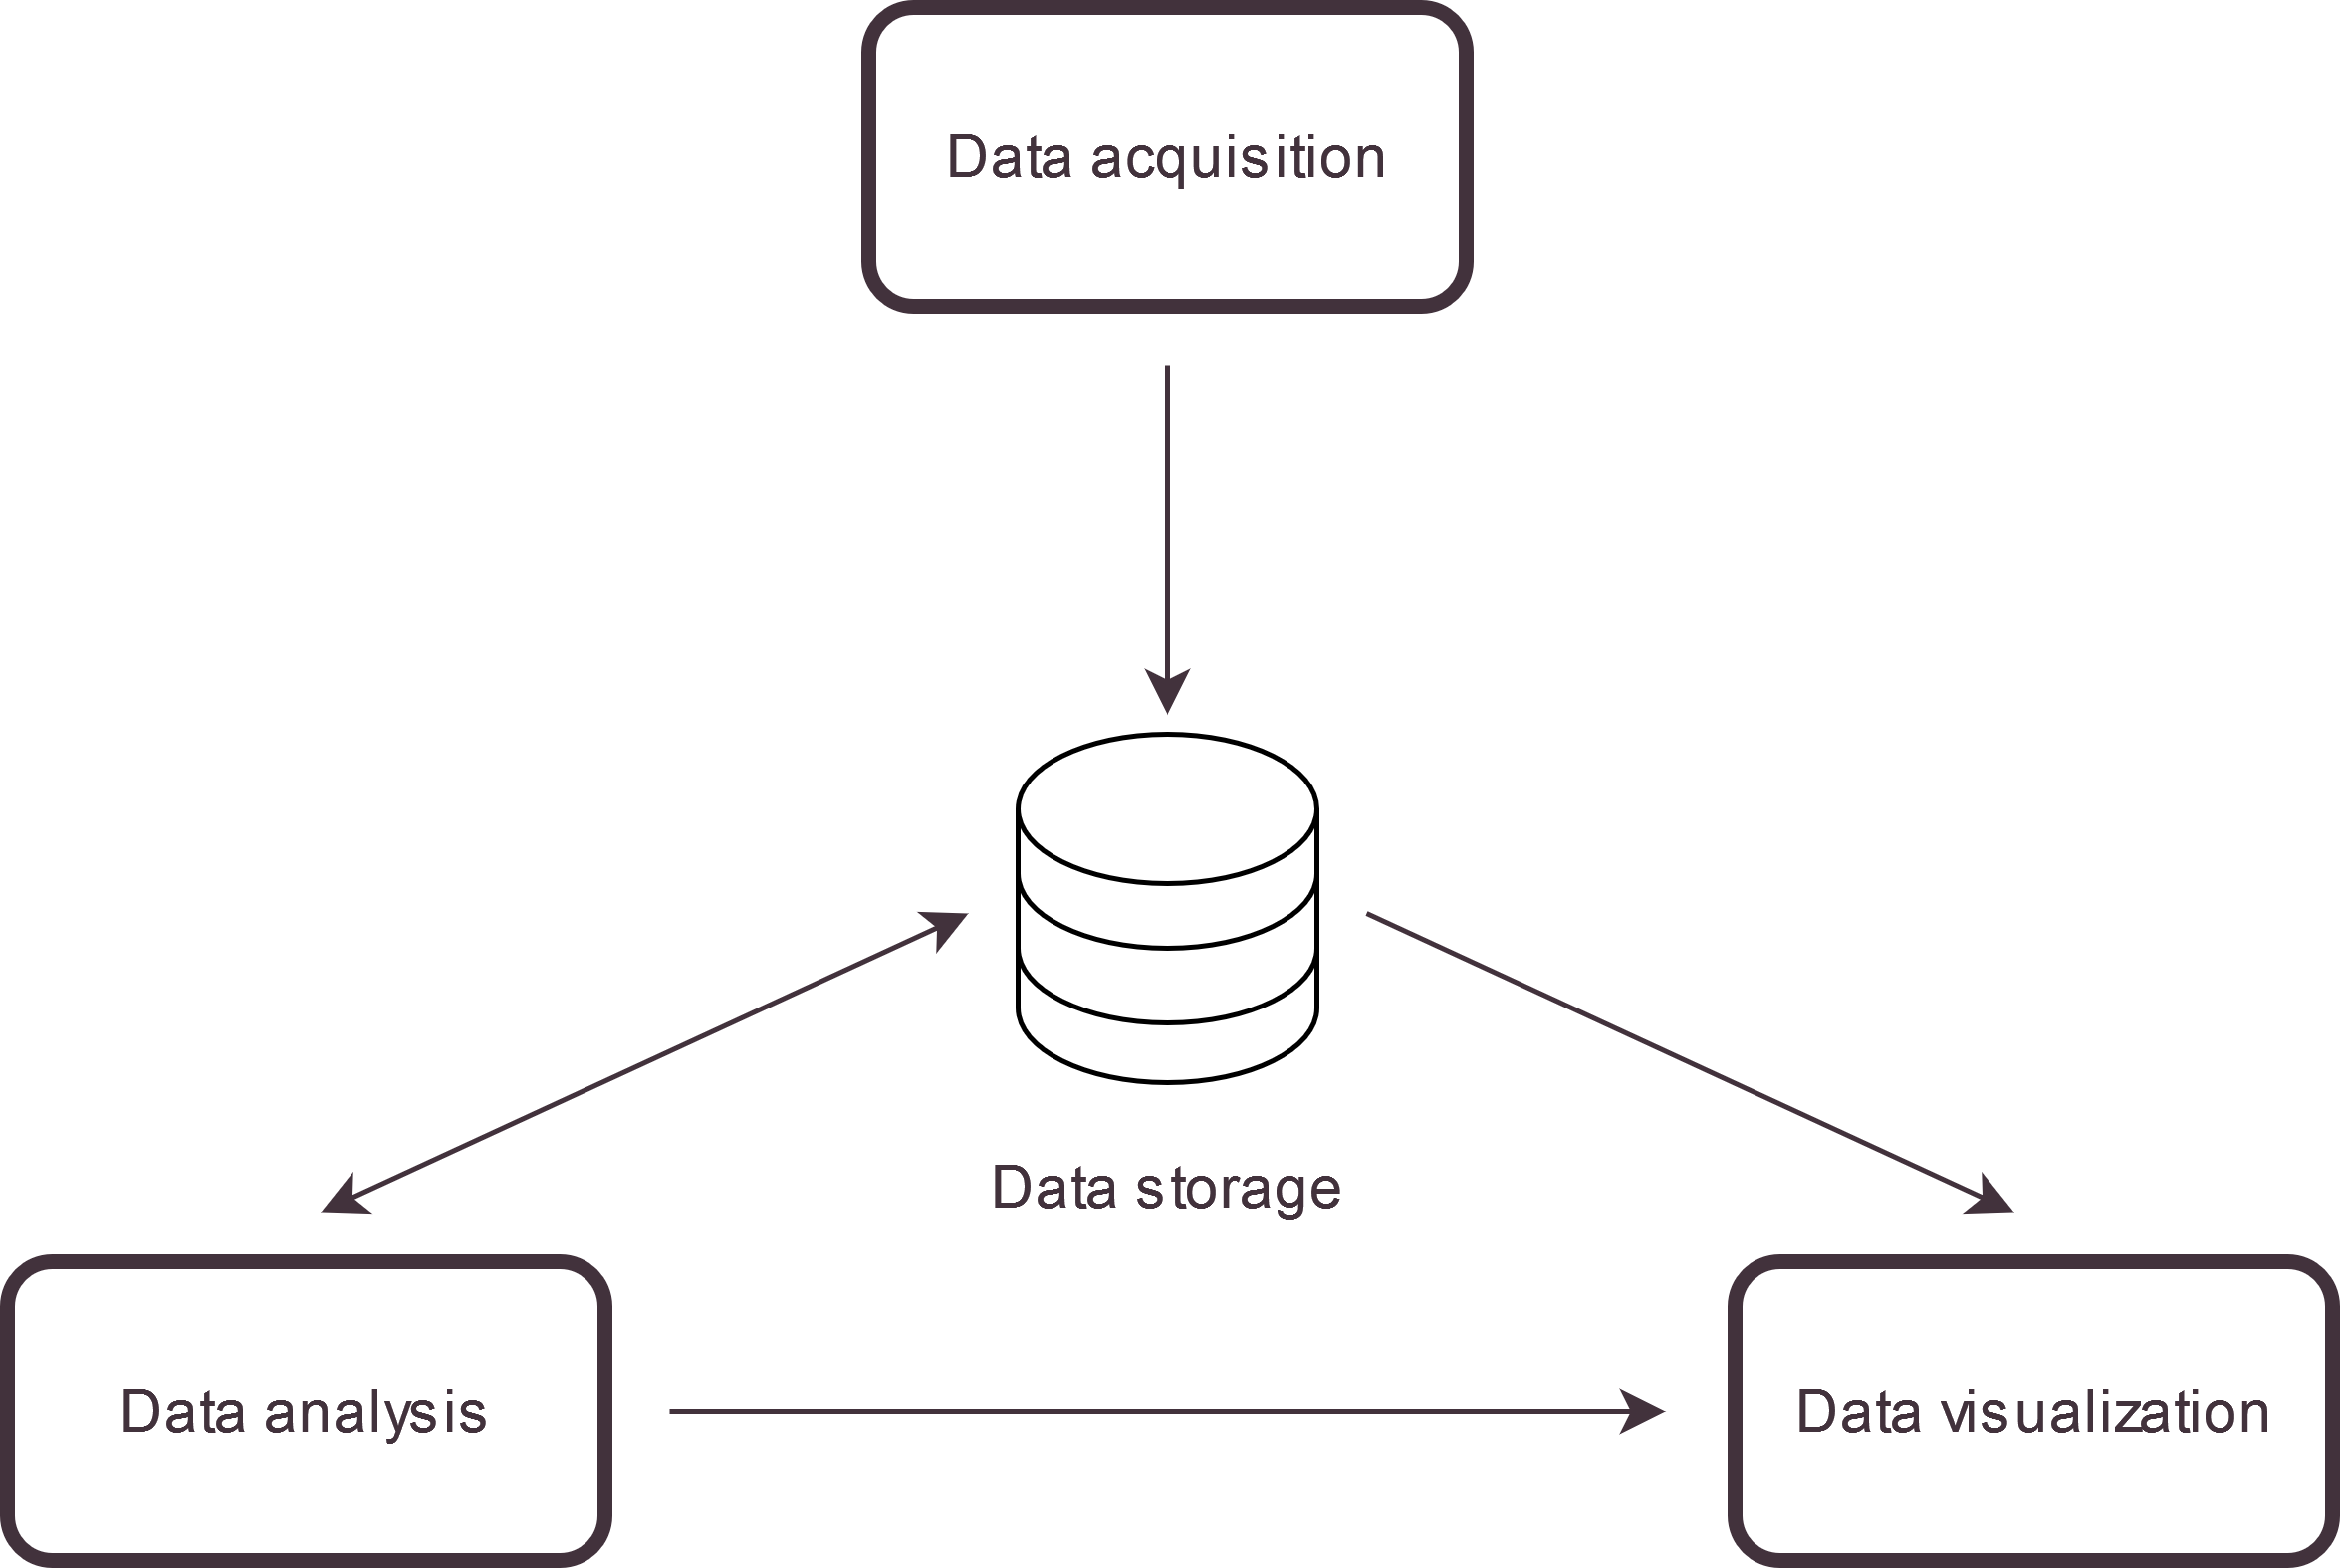
\includegraphics[width=0.85\textwidth]{Imagenes/Chapter_3/structure.png}
    \caption{Estructura base de la aplicación.}
    \label{fig:aprsint-logo}
\end{figure}

Cada uno de estos módulos será explicado en detalle en el capítulo siguiente.